\chapter{Supplemental Material for 
Chapter~\ref{chapter_umap}}

\begin{figure}[htbp]
\centering
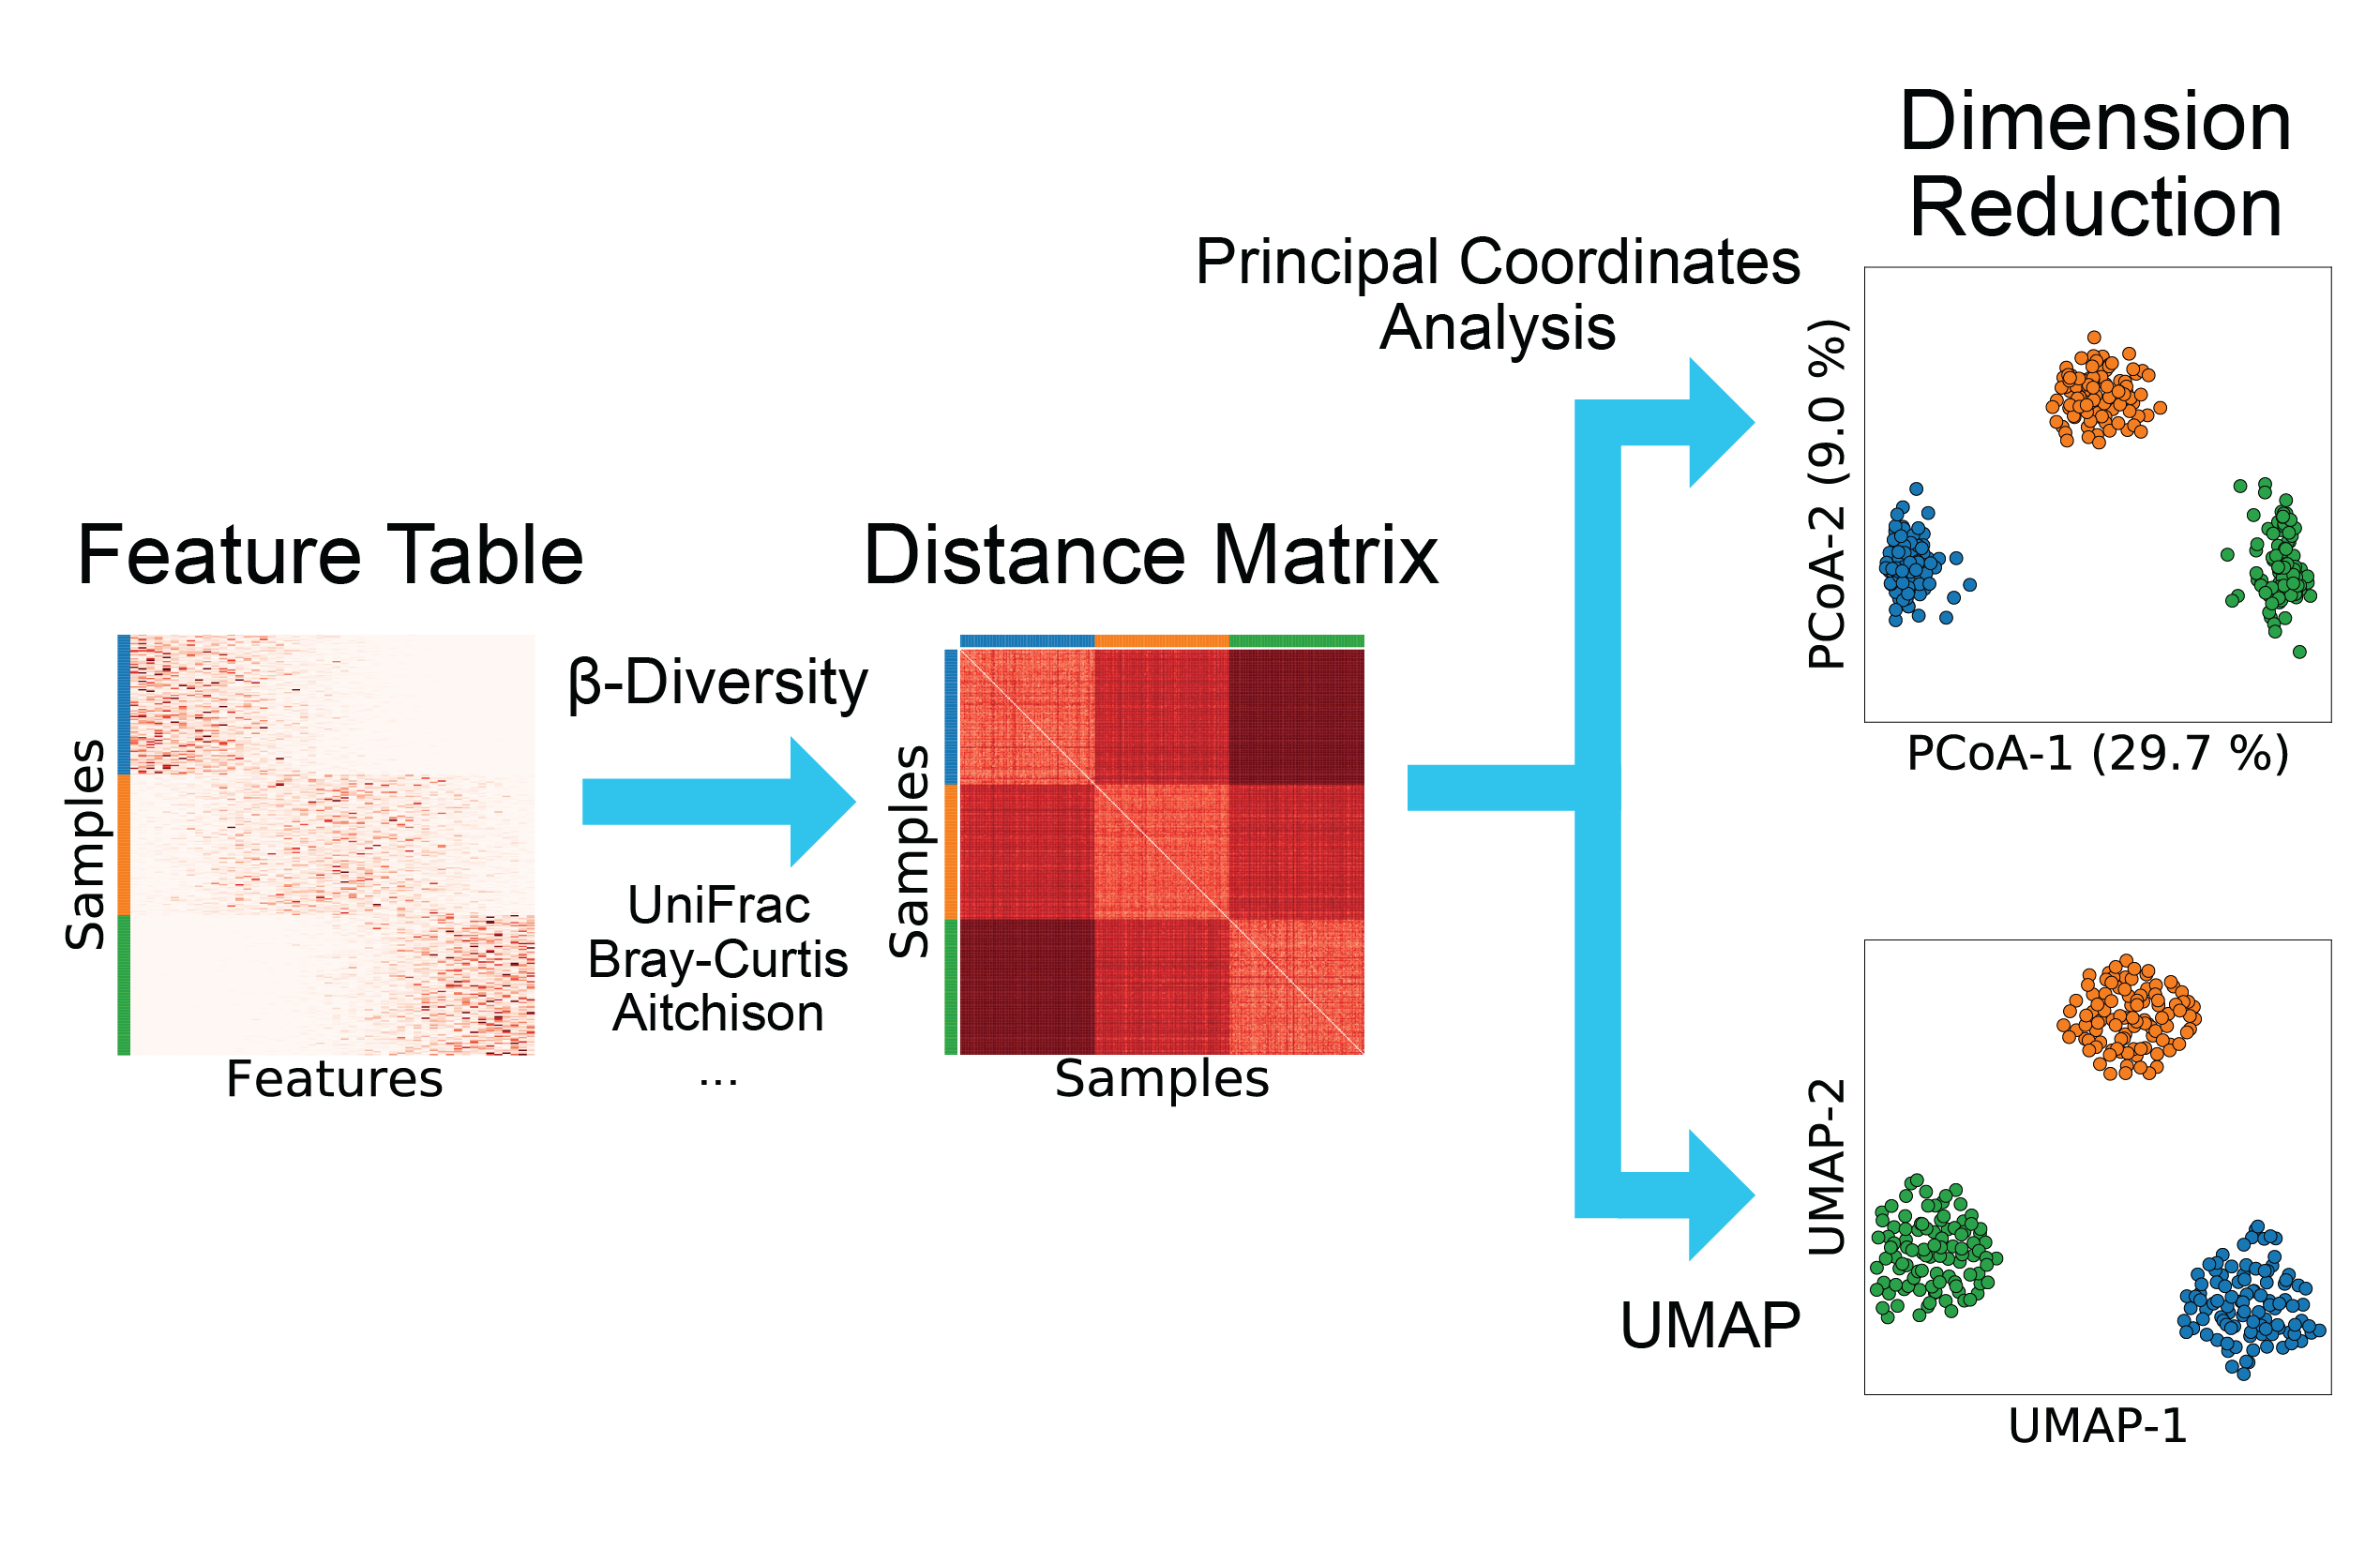
\includegraphics[width=\textwidth]{umap-figures/figureS01.png}
\caption[Graphical abstract.]{\textbf{Graphical abstract.} UMAP can operate on distance matrices of arbitrary distance metrics (UniFrac, Bray-Curtis, Aitchison), similarly to PCoA.}
\label{umap_figS1}
\end{figure}

\begin{figure}[htbp]
\centering
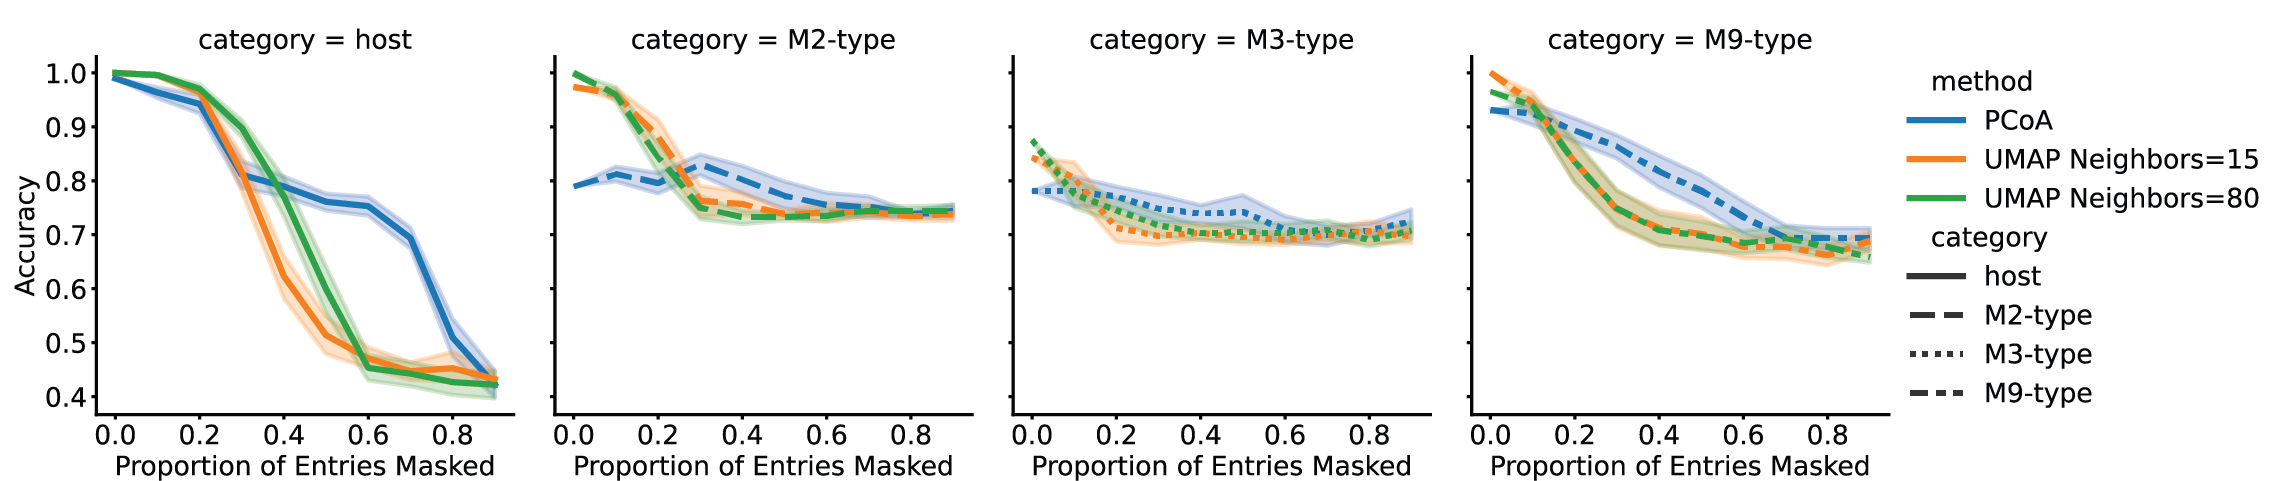
\includegraphics[width=\textwidth]{umap-figures/figureS02.png}
\caption[Simulated missing data on keyboard study.]{\textbf{Simulated missing data on keyboard study.} A proportion of the entries of the table were randomly masked (20 repetitions per ablation level) from the feature table, and dimensionality reduction followed by LDA was run on each of the tables. Host accuracy is the accuracy for identifying the correct subject. The subject-type accuracies are specific sample-type accuracies specific to the individual.}
\label{umap_figS2}
\end{figure}

\begin{figure}[htbp]
\centering
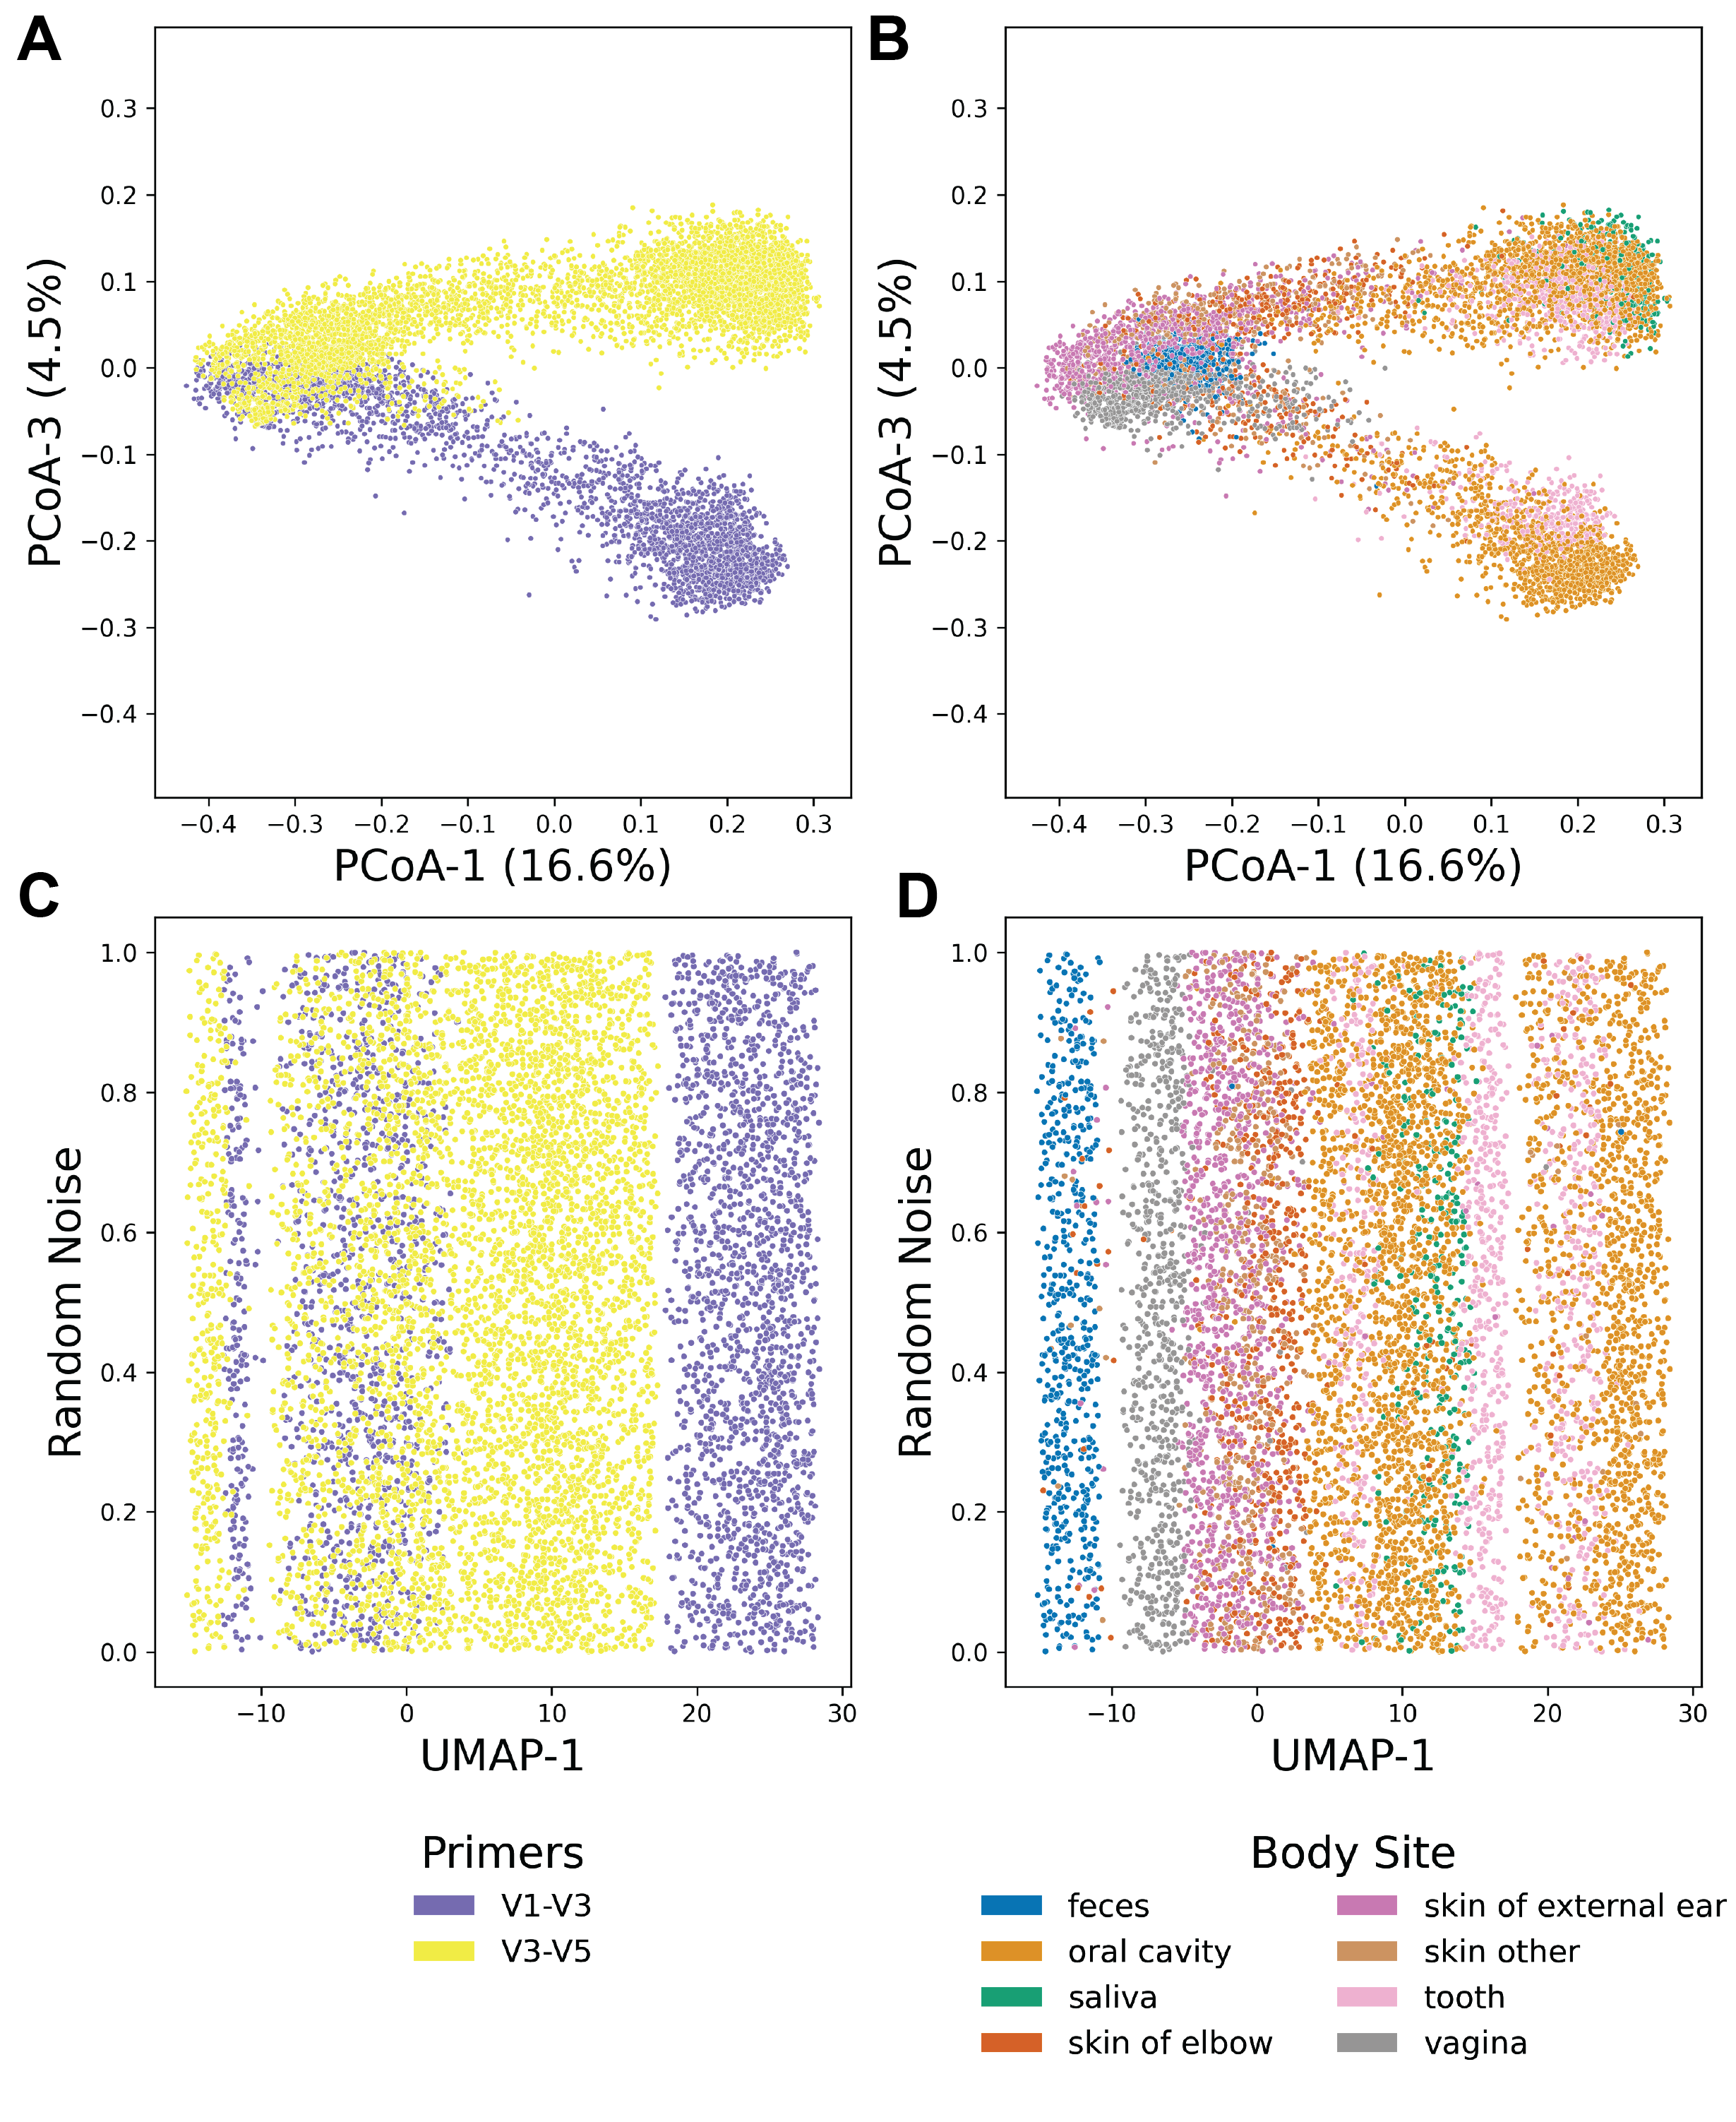
\includegraphics[width=\textwidth]{umap-figures/figureS03.png}
\caption[ Alternative views for PCoA and UMAP comparison on 8,280 samples from the Human Microbiome Project (HMP).]{\textbf{ Alternative views for PCoA and UMAP comparison on 8,280 samples from the Human Microbiome Project (HMP).} (A) PCoA-3 shows separation by primers and (B) some symmetry of sample site by primer. (C) UMAP separates the primers as well as (D) body sites in only one dimension.}
\label{umap_figS3}
\end{figure}


\chapter{Supplemental Material for Chapter~\ref{chapter_host_filtering}}

\begin{figure}[htbp]
\centering
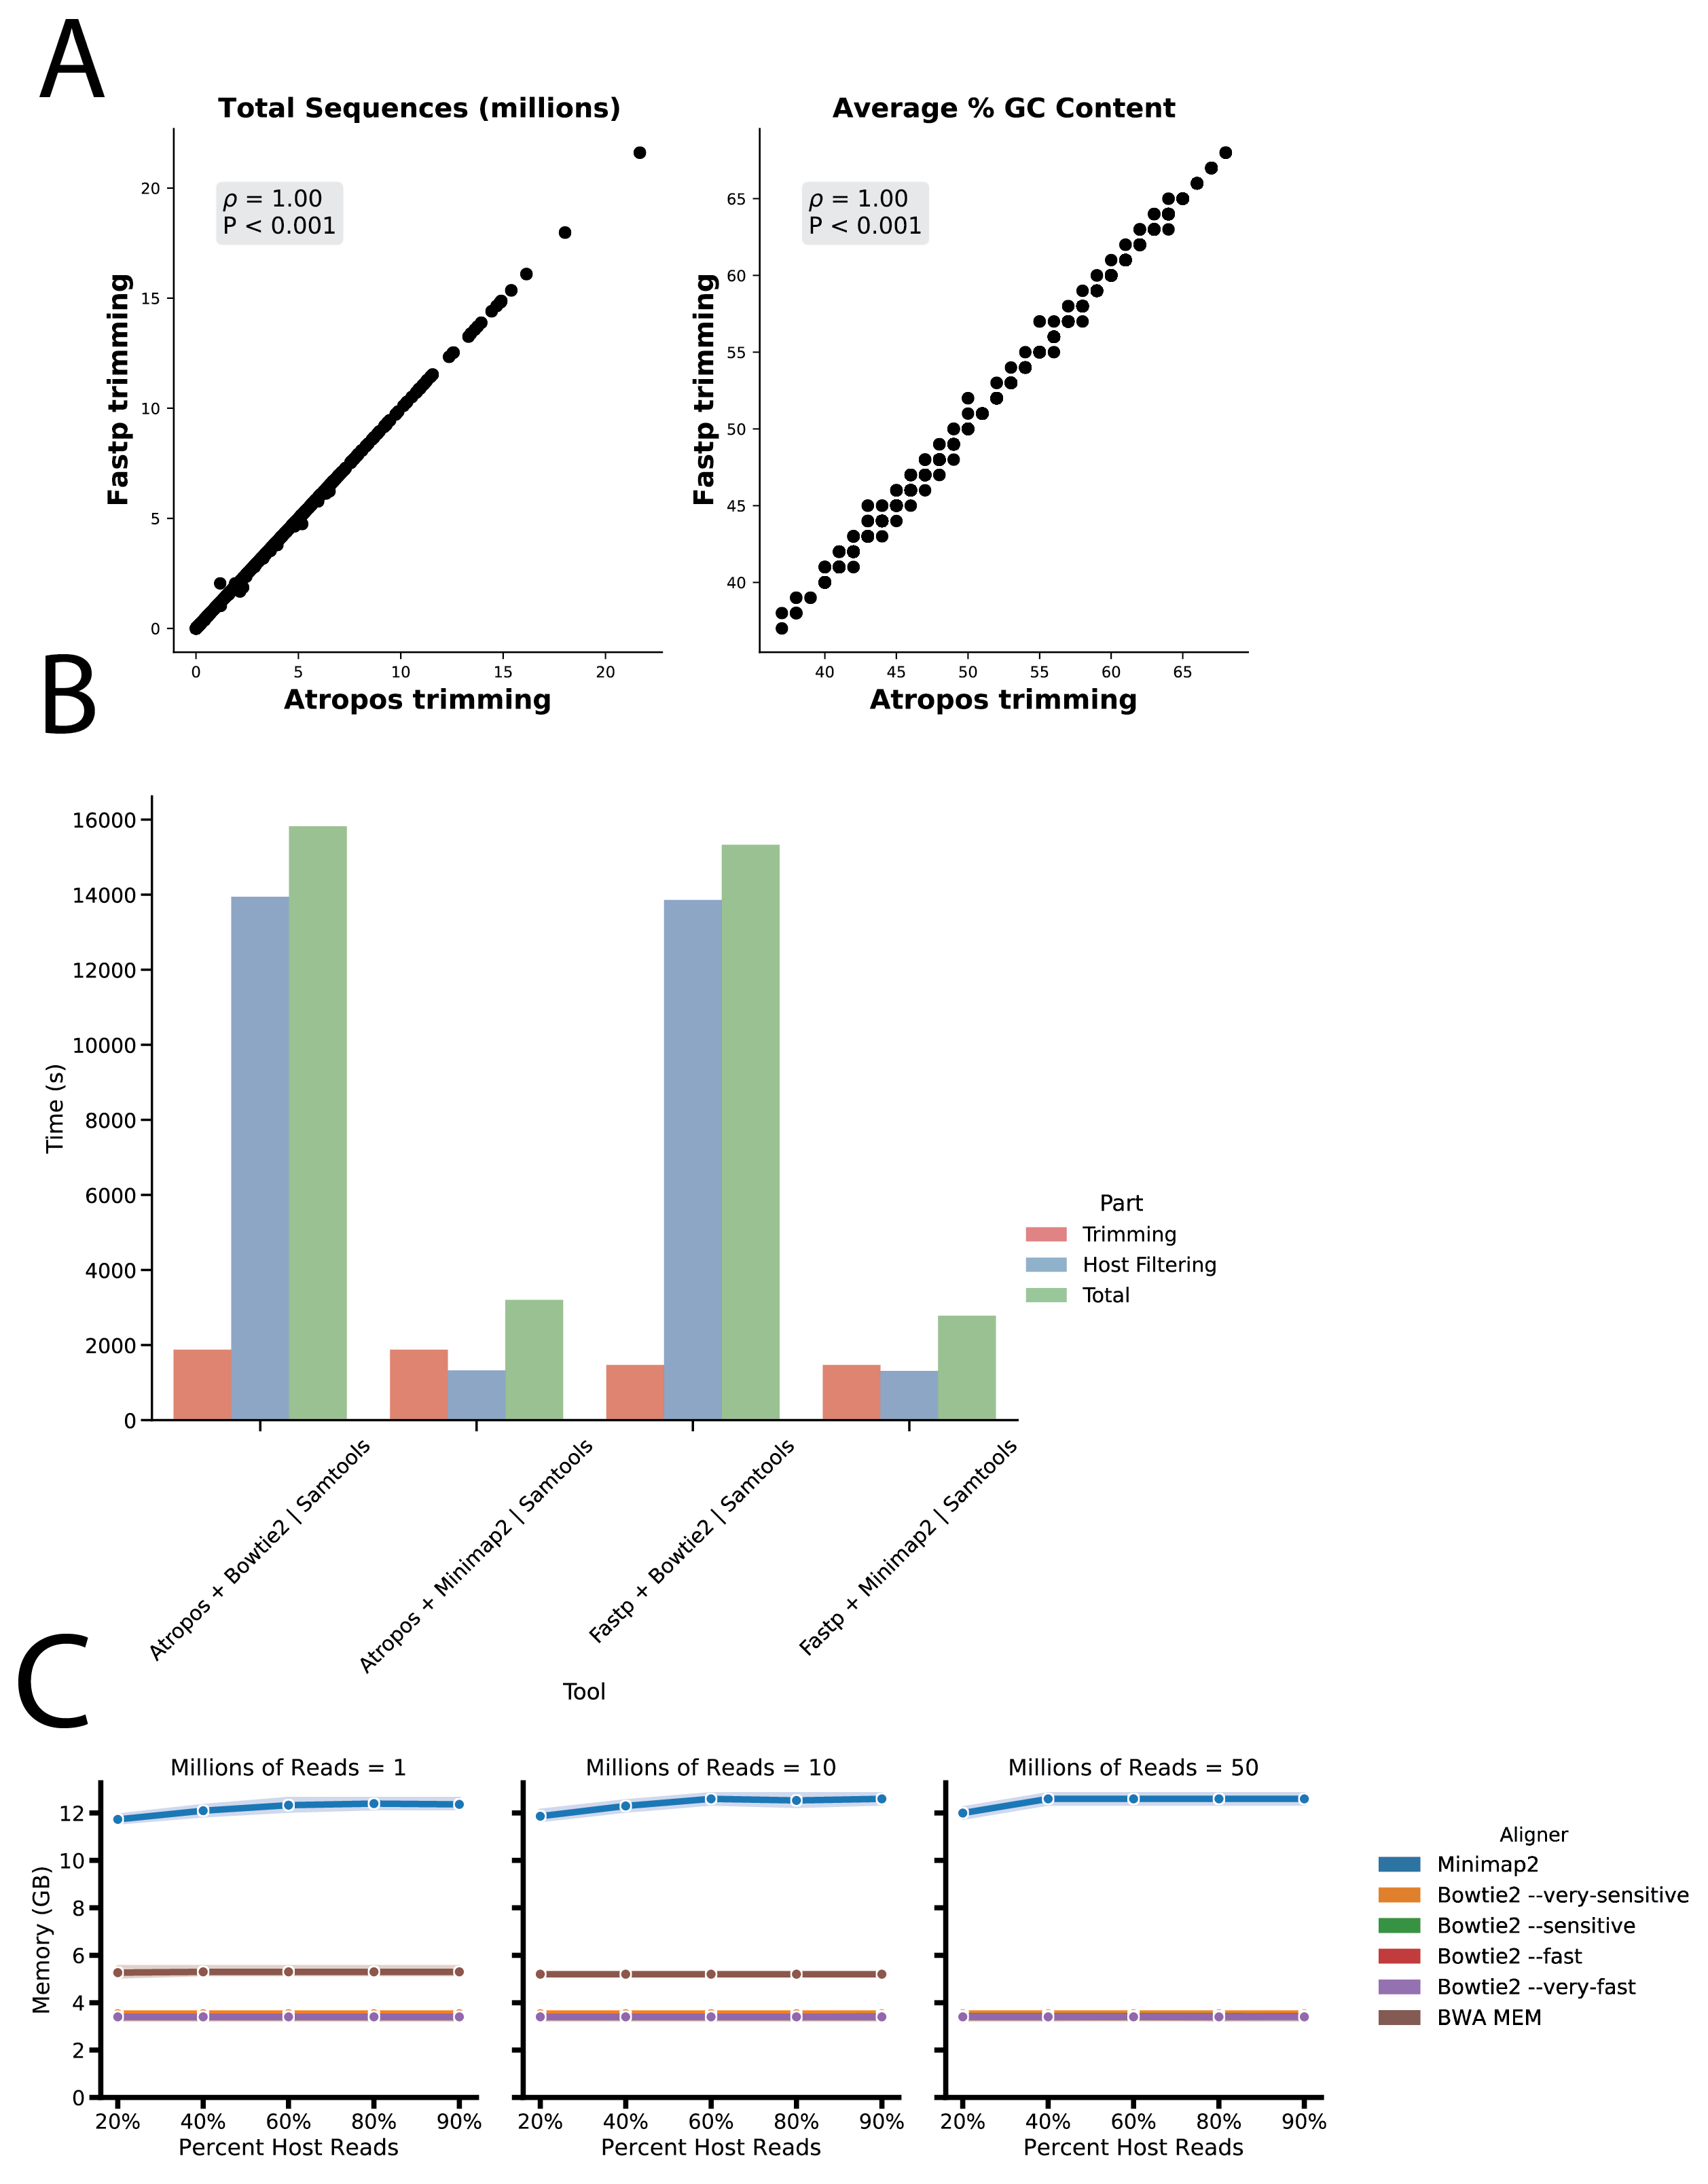
\includegraphics[width=0.9\textwidth]{host-filtering-figures/figureS01.png}
\caption[Comparison of total processing pipeline. ]{\textbf{Comparison of total processing pipeline. } (A) Comparison of trimming results on the kit extraction samples from reference 3. Each point represents the content of one sample. (B) Runtime (seconds) (y axis) between Fastp/Minimap2 and Atropos/Bowtie2 (x axis). (C) Peak memory usage for aligners using the CAMI-Sim simulated reads.}
\label{host_filtering_figS1}
\end{figure}

\begin{figure}[htbp]
\centering
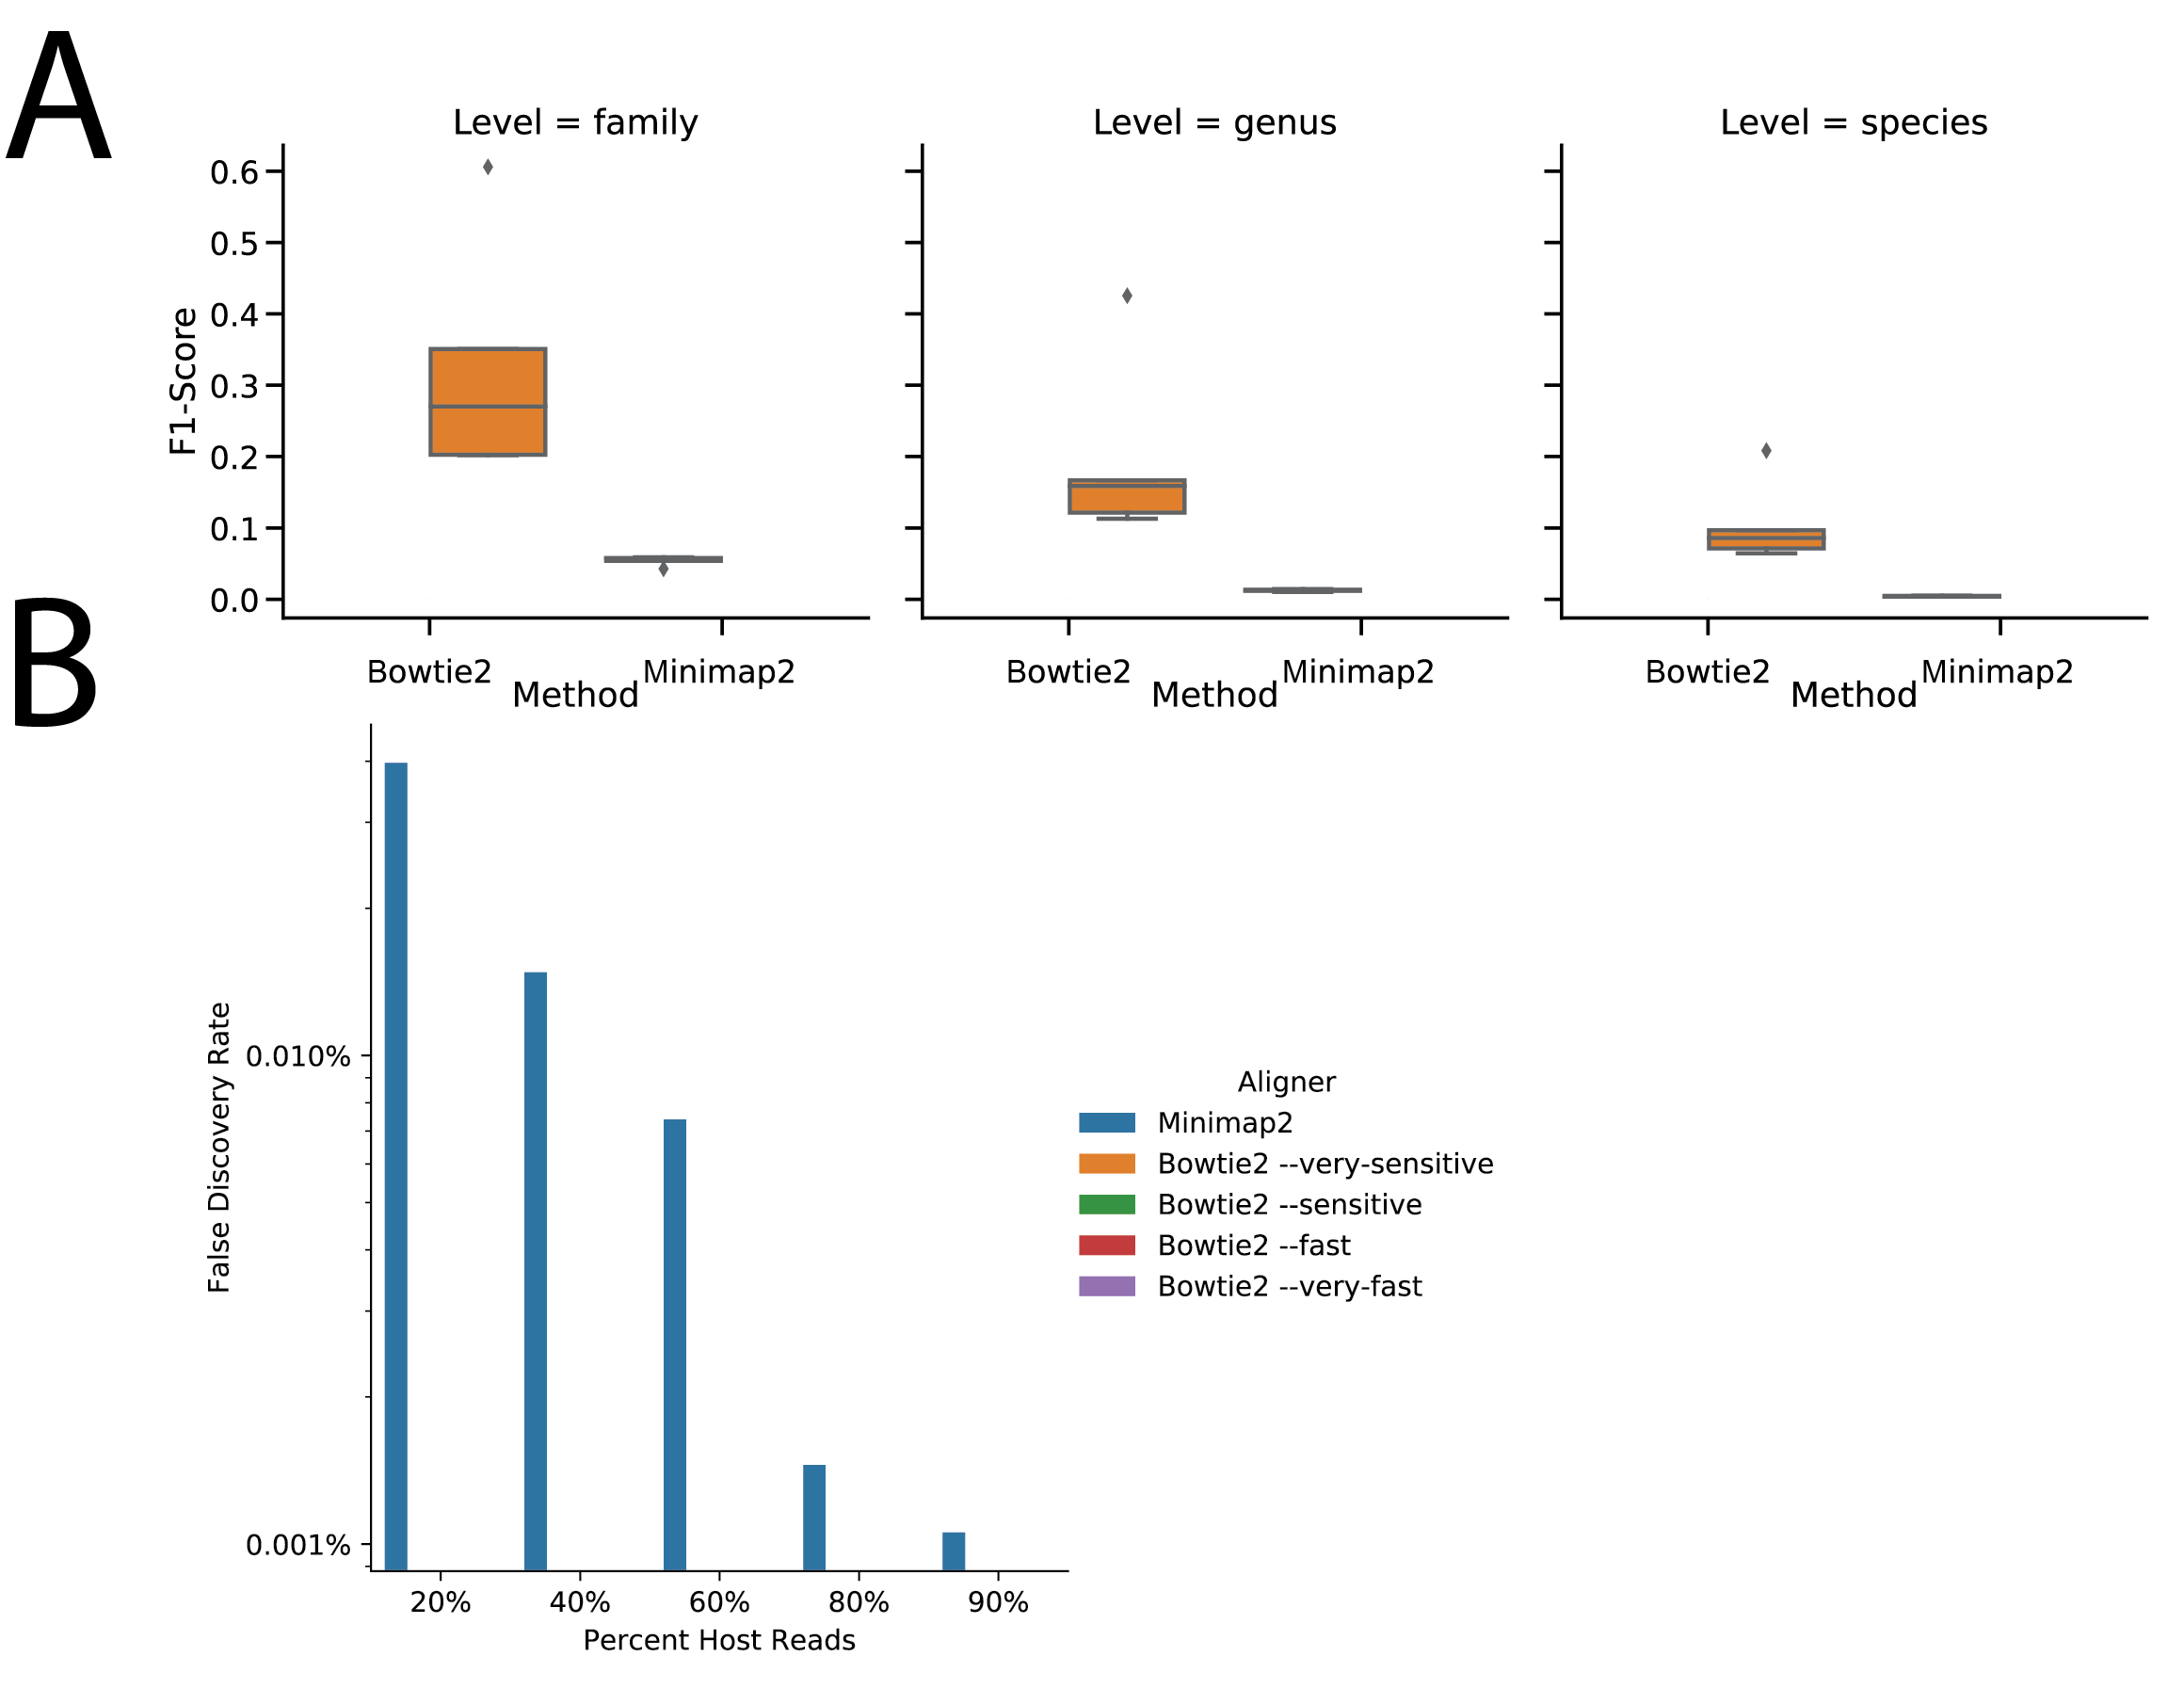
\includegraphics[width=\textwidth]{host-filtering-figures/figureS02.png}
\caption[Minimap2 gives poor taxonomic assignment compared to commonly used methods.]{\textbf{Minimap2 gives poor taxonomic assignment compared to commonly used methods.} (A) Comparison of Minimap2 and Bowtie2 (default) by F1 scores of taxon identification at family, genus, and species levels. (B) False discovery rate of Minimap2 and Bowtie2 for host filtering on the simulation data from Figure~\ref{host_filtering_fig1}A and B. Bars not shown indicate a value of 0.}
\label{host_filtering_figS2}
\end{figure}

\begin{table}

\caption[Refseq Assembly Accessions for Genomes included in simulation data]{Refseq Assembly Accessions for Genomes included in simulation data.}
\label{host_filtering_table_S1}

\centering
\begin{tabular}{ll} \hline
organism\_name          & refseq\_assembly\_accession  \\ 
\hline
\textit{Bacillus subtilis}       & GCF\_000009045.1             \\
\textit{Listeria monocytogenes}  & GCF\_000196035.1             \\
\textit{Staphylococcus aureus}   & GCF\_000013425.1             \\
\textit{Enterococcus faecalis}   & GCF\_000415185.1             \\
\textit{Lactobacillus fermentum} & GCF\_000010145.1             \\
\textit{Salmonella enterica}     & GCF\_000195995.1             \\
\textit{Escherichia coli }       & GCF\_000008865.2             \\
\textit{Pseudomonas aeruginosa } & GCF\_000006765.1             \\
\textit{Homo sapiens}          & GCF\_000001405.39           \\ \hline
\end{tabular}

\end{table}

\begin{table}
    \caption[ Exome sequencing data summary]{ Exome sequencing data summary.}
    \label{host_filtering_table_S2}
    \centering
    Table~\ref{host_filtering_table_S2} can be downloaded \href{https://journals.asm.org/doi/suppl/10.1128/msystems.01378-21/suppl_file/msystems.01378-21-st002.xlsx}{here}.
\end{table}
